\documentclass[11pt]{article}
\usepackage{amssymb}
\usepackage{latexsym}
\usepackage{float}
\usepackage{graphicx}
\usepackage{booktabs}
\usepackage{rotating}
\usepackage{lscape}
\usepackage{amsmath}
\usepackage{xeCJK}
\usepackage{indentfirst}
\usepackage{multirow}
\usepackage[colorlinks,linkcolor=blue,citecolor=blue]{hyperref}
\setcounter{MaxMatrixCols}{10}
\oddsidemargin=0.3in \textwidth=6.0in
\renewcommand\arraystretch{0.5}
\renewcommand{\baselinestretch}{1.3}
\renewcommand{\theequation}{\thesection.\arabic{equation}}
\setcounter{equation}{0}
\title{The Effect of TCJA 2017 on Capital Investment Across Different Industries in the US}
\author{Yizhe Huang\footnote{YizheHuang2025@u.northwestern.edu}}
\date{\today}
\begin{document}
\maketitle
\begin{abstract}  
This study examines the impact of the Tax Cuts and Jobs Act (TCJA) of 2017 on capital investment across various industries in the United States. By reducing the corporate tax rate and introducing measures such as full expensing for certain capital investments, the TCJA aimed to stimulate economic growth and enhance corporate competitiveness. However, the effects of this reform have varied significantly across industries, influenced by factors such as capital intensity and reliance on tangible versus intangible assets. Using firm-level capital investment data from 2011 to 2023 and employing a difference-in-differences framework, we find that capital-intensive firms experienced substantial increases in capital expenditures, primarily due to accelerated depreciation provisions, while non-capital-intensive firms showed limited or negative investment responses. Robustness checks confirm the persistence of these effects, and the inclusion of state and year fixed effects highlights the role of local economic conditions in moderating the impact of the TCJA. This research contributes to the literature on tax reforms by providing empirical evidence on their heterogeneous effects, offering insights for policymakers to consider industry-specific dynamics in fiscal policy design.  
\end{abstract}  
\thispagestyle{empty}
\newpage
\tableofcontents
\thispagestyle{empty}
\newpage

\section{Introduction}

The Tax Cuts and Jobs Act (TCJA) of 2017 represents a landmark reform in U.S. fiscal policy, fundamentally altering the corporate tax landscape. By reducing the corporate tax rate from 35\% to 21\%, the TCJA aimed to stimulate economic growth, enhance corporate competitiveness, and incentivize capital investment. In addition to lowering tax rates, the reform introduced a territorial tax regime and temporary full expensing for certain capital investments, reflecting its broad scope and ambitious objectives. However, the heterogeneity of U.S. industries, characterized by diverse capital structures and investment priorities, raises questions about the uniformity of its impact.

Understanding the differential effects of the TCJA across industries is essential to assess the reform's effectiveness. Industries vary significantly in their reliance on tangible versus intangible assets, their capital intensity, and their responsiveness to tax incentives. This study seeks to evaluate these heterogeneous impacts by analyzing firm-level capital investment data from 2011 to 2023. Specifically, the analysis focuses on whether capital-intensive industries benefited more substantially from the TCJA, and how state-level economic conditions and firm-specific characteristics shaped investment responses.

This paper provides a detailed examination of the heterogeneous effects of the TCJA on capital investment across U.S. industries. Using a difference-in-differences framework, the analysis highlights the role of capital intensity in shaping firms’ responses to the reform. Baseline regression results indicate that capital-intensive firms benefited significantly from the TCJA, particularly due to accelerated depreciation provisions, whereas non-capital-intensive firms showed limited or negative investment responses.

Robustness checks, including varying thresholds for capital intensity and controlling for state GDP growth, confirm the persistence of these effects. Notably, the inclusion of state and year fixed effects underscores the influence of local economic conditions and macroeconomic trends in moderating policy impacts. These findings reveal the nuanced dynamics between federal tax reforms and firm-level investment behaviors, emphasizing the need for industry-specific considerations in fiscal policy design.

This study contributes to the literature by providing empirical evidence on the differential impact of tax reforms, offering insights for policymakers aiming to balance the economic objectives of equity, efficiency, and growth across diverse industrial landscapes.


The structure of the paper is as follows. The next section provides a comprehensive review of the literature on tax reforms and corporate investment. The subsequent section outlines the theoretical framework underpinning the analysis. The data sources and methodological approach are detailed in the fourth section, followed by the presentation of empirical findings. The final sections discuss the implications of the results and conclude with recommendations for policy and future research.


\section{Literature Review}
The Tax Cuts and Jobs Act of 2017 has had a significant impact on corporate capital investment in the U.S., but its impact has varied widely by industry. However, the existing literature provides mixed descriptions of its effects, highlighting the complexity of the policy's impact on different industries.

\hyperref[crawford]{Crawford and Markarian (2024)} find that the TCJA stimulated capital investment, particularly in capital-intensive industries and among capital-strapped firms. U.S. firms, particularly domestic firms, experienced more significant increases in capital expenditures than their Canadian counterparts, suggesting a significant domestic impact. Meanwhile, the relatively muted response from multinationals suggests that global tax considerations may have diluted the intended effect. From this, we wanted to explore whether capital investment varies across industries in the United States.

We first thought that capital-intensive industries would be most likely to be affected, but \hyperref[gale]{Gale et al. (2024)} emphasize that the TCJA does not have a consistent impact on different types of investment. While investment in equipment and construction increased slightly, investment in intellectual property increased significantly. This suggests that industries focusing on intangible assets such as technology and innovation are better placed to benefit from tax cuts. The weak growth in tangible investment may reflect longer payback periods and uncertainty, making these industries less responsive than those with more immediate benefits.

Other studies have given similar results, with \hyperref[wagner]{Wagner, Zeckhauser, and Ziegler (2020)} illustrating the differential impact of the TCJA on the effective tax rate (ETR) across industries, leading to different results. Industries such as medical devices and electronics clearly benefit, leading to increased investment, while industries such as real estate and printing face unexpected increases in effective tax rates, which dampen investment. This discrepancy highlights the mismatch between policy intentions and their actual impact on certain industries.

In sum, the relevant literature suggests that the TCJA has had different impacts on different industries and different types of investment. Capital-intensive and IP-driven industries have benefited significantly, while industries such as real estate and those with high unexpected tax burdens have faced challenges. These mixed results highlight the limitations of a one-size-fits-all approach to tax policy and suggest that the effectiveness of such reforms depends on the specific characteristics and needs of each industry.

\section{Theory}

The optimal investment \( I \) satisfies the following profit maximization condition:
\begin{equation}
\Pi = \Pi_1 + \beta \cdot \Pi_2
\end{equation}

\noindent where:
\begin{equation}
\Pi_1 = (1 - \tau) R_1 - C(I) + \omega \tau I,
\end{equation}
\begin{equation}
\Pi_2 = (1 - \tau) R_2,
\end{equation}
\begin{equation}
C(I) = \alpha I^2,
\end{equation}
\begin{equation}
R(K) = A K^\theta,
\end{equation}
\begin{equation}
K_2 = (1 - \delta) K_1 + I.
\end{equation}

\noindent \textbf{Explanation of Terms:}
\begin{itemize}
    \item \( \beta \): Discount factor for future profits (\( 0 < \beta < 1 \)).
    \item \( R(K) \): Capital revenue function, exhibiting diminishing returns (\( 0 < \theta < 1 \)).
    \item \( C(I) \): Quadratic investment cost function (\( \alpha > 0 \)).
    \item \( K_1, K_2 \): Current and future capital, adjusted by depreciation (\( 0 < \delta < 1 \)).
    \item \( \omega \): Tax deduction rate (\( 0 \leq \omega \leq 1 \)).
    \item \( \tau \): Tax rate (\( 0 \leq \tau \leq 1 \)).
\end{itemize}

\subsection{First-Order Condition}

The first-order condition for optimal investment is:
\begin{equation}
-2\alpha I + \omega \tau + \beta (1 - \tau) A \theta \left[(1 - \delta) K_1 + I\right]^{\theta - 1} = 0.
\end{equation}

\noindent This condition balances:
\begin{itemize}
    \item The marginal cost of investment (\( -2\alpha I \)).
    \item Tax deduction benefits (\( \omega \tau \)).
    \item Future marginal returns on investment:
    $$
    \beta (1 - \tau) A \theta \left[(1 - \delta) K_1 + I\right]^{\theta - 1}.
    $$
\end{itemize}

\subsection{Sensitivity Analysis}

\subsubsection{Effect of Tax Deductions (\( \frac{dI}{d\omega} \))}

Differentiating the first-order condition with respect to \( \omega \), we get:
\begin{equation}
\frac{dI}{d\omega} = \frac{-\tau}{-2\alpha + \beta (1 - \tau) A \theta (\theta - 1) \left[(1 - \delta) K_1 + I\right]^{\theta - 2}}.
\end{equation}

\noindent \textbf{Sign Analysis:}
\begin{itemize}
    \item The numerator (\( -\tau \)) is non-positive (\( \tau \geq 0 \)).
    \item The denominator is negative, as \( -2\alpha < 0 \) and \( \theta (\theta - 1) < 0 \).
\end{itemize}
Thus:
$$
\frac{dI}{d\omega} \geq 0,
$$
implying that higher tax deductions (\( \omega \)) increase investment.

\subsubsection{Effect of Elasticity (\( \frac{dI}{d\theta} \))}

Differentiating with respect to \( \theta \), we obtain:
\begin{equation}
\frac{dI}{d\theta} = \frac{\beta (1 - \tau) A \left[(1 - \delta) K_1 + I\right]^{\theta - 1} \left[1 + \theta \ln \left((1 - \delta) K_1 + I\right)\right]}{2\alpha}.
\end{equation}

\noindent \textbf{Sign Analysis:}
\begin{itemize}
    \item The numerator is positive for \( 0 < \theta < 1 \) and \( \ln \left((1 - \delta) K_1 + I\right) \geq 0 \), reflecting that higher \(\theta\) increases the marginal productivity of capital.
    \item The denominator (\( 2\alpha \)) is positive as \(\alpha > 0\).
\end{itemize}
Thus:
$$
\frac{dI}{d\theta} > 0,
$$
indicating that higher elasticity (\( \theta \)) leads to increased investment by enhancing capital productivity.

\subsubsection*{Implication for Capital Intensity}

The sensitivity of investment to \(\theta\) (\( \frac{dI}{d\theta} \)) has important implications for capital intensity. In a production function of the form \( R(K) = A K^\theta \), the parameter \(\theta\) reflects the responsiveness of output to changes in capital. For more capital-intensive firms:
\begin{itemize}
    \item A higher \(\theta\) indicates a greater reliance on capital for output, amplifying the marginal returns to additional investment.
    \item This implies that capital-intensive industries are more sensitive to changes in \(\theta\), as their production is heavily dependent on the effective utilization of capital stock.
\end{itemize}

\noindent \textbf{Policy Insight:} The heterogeneity in responses to \(\theta\) underscores the varying effects of tax reforms (e.g., the TCJA) across industries with different capital intensities. For capital-intensive industries, a higher \(\theta\) magnifies the benefits of policies aimed at reducing the cost of capital, such as accelerated depreciation provisions. Conversely, less capital-intensive firms may experience weaker investment responses, as their production relies more on non-capital inputs (e.g., labor or intangible assets).



\section{Data}
Our study utilizes data from Capital IQ by S\&P Global, a highly reputable source widely used in financial and economic research, providing detailed microeconomic data. Since we study the 2017 TCJA, we select data that cover six years on either side of the TCJA, spanning from 2011 to 2023.

\subsection{Key Variables}
The dataset includes essential microeconomic data for publicly listed US companies:

\begin{itemize}
    \item \textbf{Geographic Information:} City and state details enable regional analyses, allowing the study of location-specific impacts.
    \item \textbf{Industry Classification:} The NAICS industry code is essential in this study, as it allows industry-specific comparisons and controls. Understanding industry dynamics is key to evaluating the varied impact of the Tax Cuts and Jobs Act in all sectors.
    \item \textbf{Other Firm-Specific Data:} Variables such as leverage ratio, return on assets (ROA), price-to-book (P/B) ratio and other financial metrics are included to capture firm-level characteristics and performance measures.
\end{itemize}

\begin{table}[htbp]
\centering
\caption{Variable Definitions}
\label{tab:variables}
\begin{tabular}{ll}
\toprule
\textbf{Variable}       & \textbf{Description} \\ 
\midrule
Capex\_Value            & Capital expenditures \\
ROA                     & Return on assets \\
TOTAL\_REV              & Total revenue \\
ASSET\_TURNS            & Asset turnover ratio \\
RETAINED\_EARN\_RESV    & Retained earnings reserve \\
TANG\_ASSETS            & Tangible assets \\
CASH\_EQUIV             & Cash and cash equivalents \\
Leverage                & Debt-to-equity ratio \\
RD\_EXP\_FN             & R\&D expenditures \\
PBV\_PERIOD\_END        & Price-to-book ratio \\
NAICS\_CODE             & Industry classification code \\
Industry\_Group         & Broad industry group \\
Finance\_Sub\_Group     & Subcategories in finance \\
State                   & U.S. state \\
Year                    & Year of observation \\
GeoName                 & Geographic name \\
Total\_GDP              & State GDP \\
Total\_Assets           & Aggregate bank assets \\
Bank\_Type              & Bank classification \\
\bottomrule
\end{tabular}
\end{table}
















\subsection{Data Processing and Handling}
The data processing workflow includes several key steps to ensure reliability and relevance for analysis.

\subsubsection{Categorization and Redistribution of Local Banks' Assets}

To accurately evaluate the impact of banks on state-level economic indicators, we classified banks into three categories based on their operational scale:
\begin{itemize}
    \item \textbf{Nation-wide Banks:} Large banks operating across multiple states, such as JPMorgan Chase and Bank of America.
    \item \textbf{Regional Banks:} Banks primarily serving specific regions, such as Comerica and M\&T Bank.
    \item \textbf{Local Banks:} Community-focused banks with limited geographic reach, focusing on localized economic activities.
\end{itemize}

This classification was necessary because the capital expenditures (CapEx) of large banks are typically recorded in the state where their headquarters are located. For example, the CapEx of nation-wide banks headquartered in New York results in disproportionately high recorded values for that state, even though their economic activities span multiple states. This creates a misrepresentation of the actual economic impact of these banks across the states where they operate.

To address this distortion, we implemented the following adjustments:
\begin{enumerate}
    \item For local banks, tangible assets (\texttt{TANG\_ASSETS}) were aggregated by state and year to compute their direct contributions to the state economy.
    \item For regional and nation-wide banks, tangible assets were redistributed across states proportionally using the GDP ratio of each state to the total GDP of the region or the nation. This adjustment was calculated as:
    \[
    \text{Weight}_{\text{state}} = \frac{\text{GDP}_{\text{state}}}{\text{GDP}_{\text{region}}}
    \]
    Using this weight, the CapEx of regional and nation-wide banks was allocated to the states where they likely conducted economic activities.
\end{enumerate}

By redistributing CapEx based on state-level GDP, the data better aligns with the actual geographic distribution of economic activity.
















\section{Methodology}
To evaluate the effect of the Tax Cuts and Jobs Act (TCJA) on capital expenditure (\textit{CapEX}), we employ a Difference-in-Differences (DID) framework. This section outlines the data construction, econometric model, control variables, and methodological limitations.
\subsection{Data Construction}
Our data set define \textit{CapEX} as follows:
\[
CapEX_{it} = Fixed\_Asset_{it} - Fixed\_Asset_{i(t-1)} + Depreciation\ and\ Allowance_{it}
\]
where:
\begin{itemize}
    \item \(Fixed\_Asset_{it}\): Fixed assets at time \(t\),
    \item \(Fixed\_Asset_{i(t-1)}\): Fixed assets at time \(t-1\),
    \item \(Depreciation\ and\ Allowance_{it}\): Depreciation and amortization allowances at time \(t\).
\end{itemize}

The dataset combines firm-level data on fixed assets, depreciation, and financial indicators from 2011 to 2023. Firms are categorized as “capital-intensive” based on their relative tangible assets in the data set. However, the specific threshold for capital intensity remains to be defined.

\subsection{Empirical Model}
The DID model is specified as follows:
\begin{align}
CapEX_{i,t} ={} & \beta_0 + \beta_1 \cdot Post_t + \beta_2 \cdot Capital\_Intensive_i + \beta_3 \cdot Post_t \cdot Capital\_Intensive_i \nonumber \\
                & + \sum_{k=1}^K \beta_k \cdot Control_{i,k,t} + \delta_t + \delta_{\text{State}} + \epsilon_{i,t}
\end{align}

where:
\begin{itemize}
    \item \(Post_t\): A dummy variable equal to 1 for years after the implementation of TCJA, and 0 otherwise,
    \item \(Capital\_Intensive_i\): A dummy variable equal to 1 if firm \(i\) is classified as capital-intensive, and 0 otherwise,
    \item \(Control_{i,k,t}\): A vector of firm-level controls including \textit{ROA}, \textit{TOTAL\_REV}, leverage, firm size, and industry fixed effects,
    \item \(\delta_t\): Time-fixed effects capturing time-specific shocks affecting all firms,
    \item \(\delta_{State}\): State fixed effects capturing time-invariant differences across states,
    \item \(\epsilon_{it}\): The error term.
\end{itemize}

\section{Preliminary Results}
\subsection{Baseline Model with 0.7 Threshold}

In this section, we present the baseline Difference-in-Differences (DID) regression results under the 0.7 threshold for defining capital-intensive firms. The regression estimates are summarized in Table~\ref{0.7table}. Three specifications are considered:
\begin{itemize}
    \item The first specification controls for state-level fixed effects.
    \item The second specification includes year fixed effects.
    \item The third specification provides the baseline model, without state or year fixed effects.
\end{itemize}

\begin{table}[htbp]
    \centering
    \caption{Regression Results with Capital-Intensive Threshold of 0.7}
    \label{0.7table}
    \begin{tabular}{lccc}
        \toprule
        \textbf{Variable} & \textbf{State FE} & \textbf{Year FE} & \textbf{Baseline Model} \\
        \midrule
        Intercept             & -101,800*** & -109,800*** & -107,000*** \\
                              & (21,000)    & (31,700)    & (13,600)    \\
        Post                  & 31,690**    & 41,540      & 48,640***   \\
                              & (10,600)    & (26,700)    & (9,723)     \\
        Post\_CapitalIntensive & -30,210     & -67,970***  & -71,160***  \\
                              & (24,300)    & (22,600)    & (22,900)    \\
        ROA                   & -0.032***   & -0.054      & -0.057      \\
                              & (0.009)     & (0.093)     & (0.085)     \\
        TOTAL\_REV            & -0.050***   & -0.048***   & -0.047***   \\
                              & (0.006)     & (0.006)     & (0.006)     \\
        ASSET\_TURNS          & -6,687      & -24,200     & -24,570     \\
                              & (10,900)    & (15,600)    & (15,400)    \\
        CASH\_EQUIV           & -0.005**    & -0.005**    & -0.005**    \\
                              & (0.002)     & (0.002)     & (0.002)     \\
        leverage              & 358         & 59          & 52          \\
                              & (730)       & (956)       & (939)       \\
        RD\_EXP\_FN           & 0.350***    & 0.316***    & 0.322***    \\
                              & (0.059)     & (0.055)     & (0.056)     \\
        PBV\_PERIOD\_END      & 608***      & 320***      & 317***      \\
                              & (117)       & (75)        & (73)        \\
        \midrule
        Observations          & 2,639       & 2,639       & 2,639       \\
        R-squared             & 0.511       & 0.370       & 0.369       \\
        Adj. R-squared        & 0.503       & 0.365       & 0.366       \\
        \bottomrule
    \end{tabular}
    \begin{flushleft}
        \footnotesize
        Notes: Robust standard errors in parentheses. *** \(p<0.01\), ** \(p<0.05\), * \(p<0.1\).
    \end{flushleft}
\end{table}


Specifically, the inclusion of state-level fixed effects in one specification reveals substantial heterogeneity across states that significantly influences CapEx outcomes. In the general case (baseline model), the results suggest that post-TCJA, capital expenditures for capital-intensive firms increased, while non-capital-intensive firms experienced reductions in capital expenditures. This aligns with the idea that capital-intensive firms benefited more from the policy, possibly due to the accelerated depreciation provisions that favor firms with higher tangible asset investments.

However, when state-level fixed effects are introduced, the $Post\_CapitalIntensive$ coefficient changes direction, indicating that the differential effect of the TCJA on capital-intensive firms is no longer as apparent. This may suggest that much of the observed increase in capital expenditures for capital-intensive firms is driven by state-level heterogeneity, such as differences in local economic conditions, tax policies, or investment climates, which the fixed effects absorb. In other words, adding state-fixed effects reduces the variation attributed to the policy itself, making the coefficient appear less robust. Nonetheless, the baseline model provides the clearest insight into the inherent differences in how the TCJA impacted capital-intensive versus non-capital-intensive firms, highlighting the policy’s heterogeneous effects.

When year-fixed effects are included, the results provide a complementary perspective, isolating the impact of time-varying macroeconomic shocks that might have affected capital expenditures across the board during the study period. Interestingly, the inclusion of year-fixed effects slightly dampens the magnitude of the \textit{Post} coefficient but retains the differential effect observed for capital-intensive firms. This suggests that macroeconomic factors, such as general economic growth, monetary policy changes, or nationwide responses to the TCJA, played a role in shaping CapEx behaviors. However, the persistence of the $Post\_CapitalIntensive$ coefficient reinforces the conclusion that capital-intensive firms were more responsive to the TCJA, albeit in a manner that reflects their distinct investment dynamics.

The substantial change caused by adding state-level fixed effects highlights the complexity of disentangling state-level heterogeneity from federal policy impacts. Conversely, year-fixed effects underscore the importance of accounting for nationwide temporal trends, which may confound policy evaluations. Together, these specifications illustrate the nuanced interplay between firm characteristics, state-level contexts, and time-specific factors in determining the outcomes of major tax reforms like the TCJA.

\subsection{Parallel Trend Test with 0.7 Threshold}
\begin{figure}
    \centering
    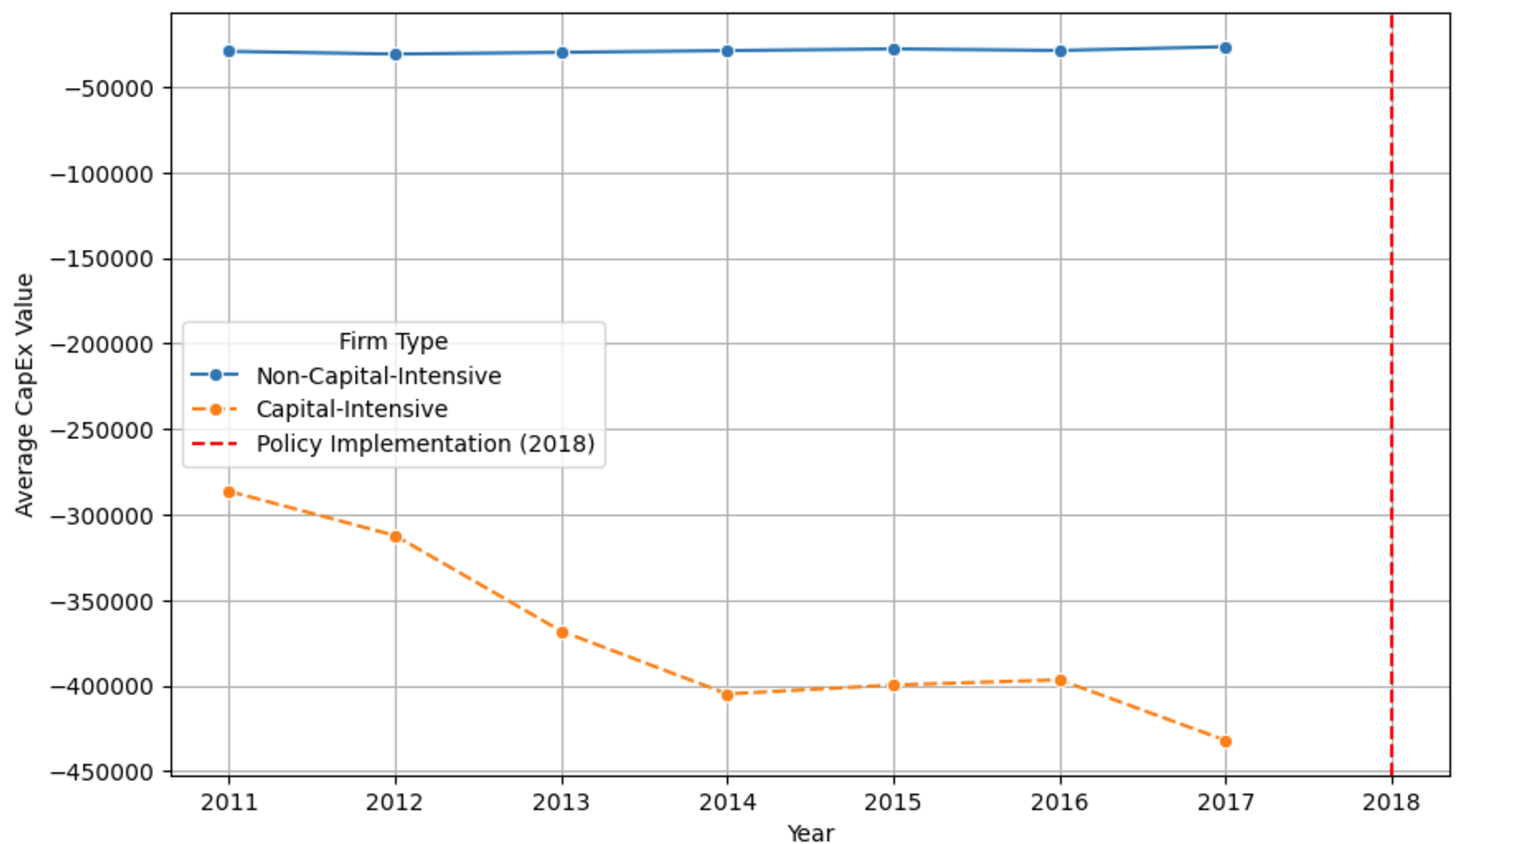
\includegraphics[width=0.75\linewidth]{b92854fdb34d09b5d1f490875bbc444.png}
    \caption{Parallel Trend Test: Pre-Treatment Trends (Capex)}
\end{figure}

To validate the Difference-in-Differences (DID) framework, we conducted a parallel trend test under the 0.7 threshold for defining capital-intensive firms. This test examines whether Capital-Intensive and Non-Capital-Intensive firms exhibited similar trends in capital expenditures (CapEx) during the pre-treatment period (2011–2017). Table~\ref{parallel_trend_table} summarizes the results of the statistical test.

The interaction terms between year dummies and the \textit{Capital\_Intensive} variable are all statistically insignificant (p-values $>$ 0.05). This indicates that there are no significant differences in the trends between Capital-Intensive and Non-Capital-Intensive firms prior to the implementation of the Tax Cuts and Jobs Act (TCJA) in 2018. Consequently, we fail to reject the null hypothesis that the two groups follow parallel trends, thereby supporting the validity of the DID framework for this analysis.

\begin{table}[htbp]
    \centering
    \caption{Statistical Parallel Trend Test Results (2011–2017)}
    \label{parallel_trend_table}
    \begin{tabular}{lccc}
        \toprule
        \textbf{Variable} & \textbf{Coefficient} & \textbf{Standard Error} & \textbf{p-value} \\
        \midrule
        Intercept & -28,900*** & 504.845 & 0.000 \\
        Capital\_Intensive & -257,400*** & 72,200 & 0.000 \\
        Year\_2012 × Capital\_Intensive & -25,890 & 104,000 & 0.804 \\
        Year\_2013 × Capital\_Intensive & -81,730 & 118,000 & 0.488 \\
        Year\_2014 × Capital\_Intensive & -118,400 & 126,000 & 0.346 \\
        Year\_2015 × Capital\_Intensive & -113,200 & 121,000 & 0.351 \\
        Year\_2016 × Capital\_Intensive & -110,200 & 118,000 & 0.352 \\
        Year\_2017 × Capital\_Intensive & -145,600 & 121,000 & 0.230 \\
        \midrule
        Observations & \multicolumn{3}{c}{11,995} \\
        R-squared & \multicolumn{3}{c}{0.038} \\
        Adj. R-squared & \multicolumn{3}{c}{0.037} \\
        \bottomrule
    \end{tabular}
    \begin{flushleft}
        \footnotesize
        Notes: Robust standard errors are reported. *** \(p<0.01\), ** \(p<0.05\), * \(p<0.1\). The model includes year dummies for 2012–2017 interacted with the \textit{Capital\_Intensive} variable.
    \end{flushleft}
\end{table}

The results from the parallel trend test validate the DID methodology used in this study, as they confirm the assumption of parallel pre-treatment trends between Capital-Intensive and Non-Capital-Intensive firms. This supports the robustness of our findings on the heterogeneous effects of the TCJA.

\section{Falsification Tests}
\subsection{Change the Threshold}
To test the robustness of our baseline model, we vary the threshold values for defining capital-intensive firms. The thresholds used include 0.1, 0.3, 0.5, 0.7, and 0.9. Table~\ref{threshold_table} summarizes the regression results for these specifications.

\begin{sidewaystable}[htbp]
    \centering
    \caption{Regression Results with Varying Capital-Intensive Thresholds}
    \label{threshold_table}
    \begin{tabular}{lccccc}
        \toprule
        \textbf{Variable} & \textbf{Threshold 0.1} & \textbf{Threshold 0.3} & \textbf{Threshold 0.5} & \textbf{Threshold 0.7} & \textbf{Threshold 0.9} \\
        \midrule
        Intercept            & -114,900*** & -114,900*** & -112,800*** & -107,000*** & -116,900*** \\
                             & (12,100)    & (12,300)    & (12,600)    & (13,600)    & (12,200)    \\
        Post                 & 50,490***   & 48,170***   & 47,990***   & 48,640***   & 40,220***   \\
                             & (13,100)    & (10,100)    & (9,862)     & (9,722)     & (10,400)    \\
        Post\_CapitalIntensive & -34,980***  & -39,550***  & -47,040***  & -71,160***  & -171,700**  \\
                             & (12,100)    & (13,000)    & (16,000)    & (22,900)    & (78,400)    \\
        TOTAL\_REV            & -0.049***   & -0.049***   & -0.048***   & -0.047***   & -0.045***   \\
                             & (0.006)     & (0.006)     & (0.006)     & (0.006)     & (0.006)     \\
        RD\_EXP\_FN           & 0.317***    & 0.323***    & 0.325***    & 0.322***    & 0.305***    \\
                             & (0.056)     & (0.056)     & (0.056)     & (0.056)     & (0.056)     \\
        PBV\_PERIOD\_END      & 361.82***   & 352.28***   & 342.20***   & 317.06***   & 339.03***   \\
                             & (72.96)     & (72.81)     & (72.91)     & (73.22)     & (70.62)     \\
        \midrule
        Observations         & 2,639       & 2,639       & 2,639       & 2,639       & 2,639       \\
        R-squared            & 0.367       & 0.368       & 0.368       & 0.369       & 0.371       \\
        Adj. R-squared       & 0.365       & 0.365       & 0.366       & 0.366       & 0.369       \\
        \bottomrule
    \end{tabular}
    \begin{flushleft}
        \footnotesize
        Notes: Robust standard errors in parentheses. *** \(p<0.01\), ** \(p<0.05\), * \(p<0.1\).
    \end{flushleft}
\end{sidewaystable}

As the threshold increases, the interaction term (\textit{Post\_CapitalIntensive}) becomes more negative, suggesting a larger increase in CapEx for Capital-Intensive firms compared to Non-Capital-Intensive firms. This result indicates that the sensitivity of the TCJA’s effects on CapEx depends on how Capital-Intensive firms are defined.

At lower thresholds, a greater proportion of firms are classified as Capital-Intensive, diluting the effect of the TCJA on these firms' CapEx. Conversely, as the threshold increases, only firms with the highest tangible asset levels are categorized as Capital-Intensive, and these firms display a substantially larger responsiveness to the policy. This trend aligns with the hypothesis that firms with higher fixed assets are more sensitive to changes in tax policy, particularly those affecting depreciation allowances.

Interestingly, the most significant effect is observed at the 0.9 threshold, where the coefficient for \textit{Post\_CapitalIntensive} indicates a pronounced increase in CapEx. This finding suggests that firms with extremely high tangible assets responded strongly to the TCJA, likely due to the accelerated depreciation provisions. However, the increased responsiveness at higher thresholds might also reflect the influence of other unobserved characteristics, such as greater financial flexibility or differing investment strategies.

Overall, this falsification test highlights the heterogeneous effects of the TCJA, driven by varying definitions of Capital-Intensive firms. These results underscore the importance of carefully selecting thresholds when studying policy impacts to ensure that relevant heterogeneity is captured and misclassification bias is minimized.

\subsection{Testing GDP Growth as a Confounder}
To assess whether state GDP growth confounds the observed effects of the TCJA on capital expenditures (CapEx), we include state GDP as a control variable in the regression model. The results, shown in Table~\ref{GDPTest}, indicate the following:

The coefficient for \(State\_GDP\) is \(0.0187\) (\(p=0.051\)), which is marginally significant, indicating that higher state GDP growth may be associated with reduced investment, as reflected by higher (less negative) CapEx values. However, the inclusion of GDP does not substantially alter the core findings: the \(Post\_CapitalIntensive\) coefficient remains significantly negative (\(-97,290\), \(p<0.01\)), confirming that capital-intensive firms increased their investments more than non-capital-intensive firms after the TCJA. The \(Post\) variable remains significantly positive (\(38,480\), \(p<0.01\)), indicating that non-capital-intensive firms reduced their investments during the same period.

This analysis suggests that while state GDP growth marginally influences investment patterns, it does not explain the heterogeneous effects of the TCJA. Capital-intensive firms still demonstrate significantly different responses compared to their non-capital-intensive counterparts.

\begin{table}[htbp]
    \centering
    \caption{Regression Results with State GDP as a Control Variable}
    \label{GDPTest}
    \begin{tabular}{lcc}
        \toprule
        \textbf{Variable} & \textbf{Coefficient} & \textbf{Standard Error} \\
        \midrule
        Intercept & -112,700*** & (25,500) \\
        Post & 38,480*** & (10,100) \\
        Post\_CapitalIntensive & -97,290*** & (34,600) \\
        State\_GDP & 0.0187* & (0.010) \\
        ROA & -0.0415 & (0.081) \\
        TOTAL\_REV & -0.0400*** & (0.010) \\
        ASSET\_TURNS & -26,140 & (20,300) \\
        CASH\_EQUIV & -0.0103** & (0.005) \\
        leverage & -184.5530 & (1,256.146) \\
        RD\_EXP\_FN & 0.2158** & (0.100) \\
        PBV\_PERIOD\_END & 278.2917*** & (106.604) \\
        \midrule
        Observations & \multicolumn{2}{c}{1,600} \\
        R-squared & \multicolumn{2}{c}{0.443} \\
        Adj. R-squared & \multicolumn{2}{c}{0.439} \\
        \bottomrule
    \end{tabular}
    \begin{flushleft}
        \footnotesize
        Notes: Robust standard errors in parentheses. *** \(p<0.01\), ** \(p<0.05\), * \(p<0.1\). Higher CapEx values indicate reduced investment.
    \end{flushleft}
\end{table}


\section{Discussion}
This study investigates the impact of the Tax Cuts and Jobs Act (TCJA) on capital expenditures of firms of different capital intensive levels with Difference-in-Difference model. Results revealed that the TCJA led to a significant increase in capital expenditures by capital-intensive firms and a decrease in investment by non-capital-intensive firms.The TCJA largely benefited firms that initially had invested heavily in tangible assets, potentially exacerbating the investment gap between sectors of the economy.

The reliability of the results is verified by a series of robustness checks. Raising the threshold for the definition of capital-intensive firms (from the 10th to the 90th percentile) does not change the direction of the observed effect. Specifically, the effect of TCJA on raising investment gradually increases as the threshold is raised. Highly capital-intensive firms experience greater increases in capital expenditures. In addition, the paper controls for state GDP growth to address potential confounding effects related to regional economic conditions. The main findings do not change substantially when state GDP is included as a control variable in the regression model. Despite the marginal association between state GDP growth and capital expenditures, the significant differential response between capital-intensive and non-capital-intensive firms persists. This suggests that the heterogeneous impact of TCJA is not simply a result of broader economic trends, but is directly related to the design and implementation of policies.

The differential impact of the TCJA raises important policy implications. First, the current tax policy framework appears to favor firms with large amounts of tangible assets, potentially leading to an uneven distribution of investment across sectors. To mitigate this imbalance, it is necessary to implement targeted tax incentives to encourage non-capital-intensive firms to increase their capital expenditures. Specific measures may include providing tax credits for equipment purchases, technological upgrades or facility expansions by non-capital-intensive firms to reduce the actual cost of investment. Second, tax policies should be adjusted to promote balanced investment across industries and mitigate the imbalance effect of the TCJA. The government can support the growth of capital investment in non-capital-intensive firms by providing them with investment subsidies, innovation grants and improved access to finance.


\newpage
\begin{thebibliography}{99}
%\bibitem{}AI-Youbi, A. Obaid., Zahed, Adnan., \& Atalar, Abdullah. (2021). International experience in developing the financial resources of universities. Springer International Publishing AG. \label{Book}



\bibitem{crawford2024effect}
Crawford, S., \& Markarian, G. (2024). The effect of the Tax Cuts and Jobs Act of 2017 on corporate investment. \textit{Journal of Corporate Finance}, 87, 102619. https://doi.org/10.1016/j.jcorpfin.2024.102619 \label{crawford}

\bibitem{gale2024sweeping}
Gale, W. G., Hoopes, J. L., \& Pomerleau, K. (2024). Sweeping changes and an uncertain legacy: The Tax Cuts and Jobs Act of 2017. \textit{Journal of Economic Perspectives}, 38(3), 3-32. https://doi.org/10.1257/jep.38.3.3 \label{gale}

\bibitem{wagner2020tax}
Wagner, A. F., Zeckhauser, R. J., \& Ziegler, A. (2020). The Tax Cuts and Jobs Act: Which firms won? Which lost? \textit{NBER Working Paper No. 27470}. National Bureau of Economic Research. https://www.nber.org/papers/w27470  \label{wagner}



\end{thebibliography}

\end{document}